\chapter{Entwicklung}\label{ch:development}

Der ursprüngliche Reed-Solomon-Code wurde 1960 von den amerikanischen Mathematikern am Licoln Laboratory des \acrshort{mit} entwickelt.
Sie veröffentlichten das Paper \textquote{Polynomial codes over certain finite fields}, in dem das neu entworfene Fehlerkorrekturverfahren beschrieben wurde.
Dabei handelt es sich um ein \acrfull{fec}, aus dem englischen \textquote{forward error correction}, welches eigenständig, ohne Rückfrage beim Absender, Fehler erkennen und beseitigen kann \cite{wickerReedSolomonCodes1994}.
Im Gegenzug dazu gibt es die Verfahren, die Fehler nur erkennen können und daraufhin fehlerhafte Daten erneut anfragen. Deshalb werden sie \acrfull{arq}-Verfahren genannt \cite{friedrichsKanalcodierung1996, geiselTutorialReedSolomonError1990}.

Durch diese Veröffentlichung wurde eine neue Klasse von \acrlong{ecc}s (\acrshort{ecc}) geschaffen. 
Reed-Solomon-Codes gehören zu der Gruppe der linearen, zyklischen Block-Codes. 
Lineare Blockcodes teilen zu codierende Daten in Blöcke mit fester Länge \(n\) und verarbeiten diese in einer endlichen algebraischen Struktur \cite{friedrichsKanalcodierung1996}. 
Bei zyklischen Codes ist diese eine endliche Algebra (siehe Abschnitt \ref{sec:galois} auf Seite \pageref{sec:galois}).
Ein Ausschnitt der Code-Hierarchie ist in Abbildung \ref{fig:eccHierarchy} dargestellt.

\begin{figure}[ht]
	\centering
	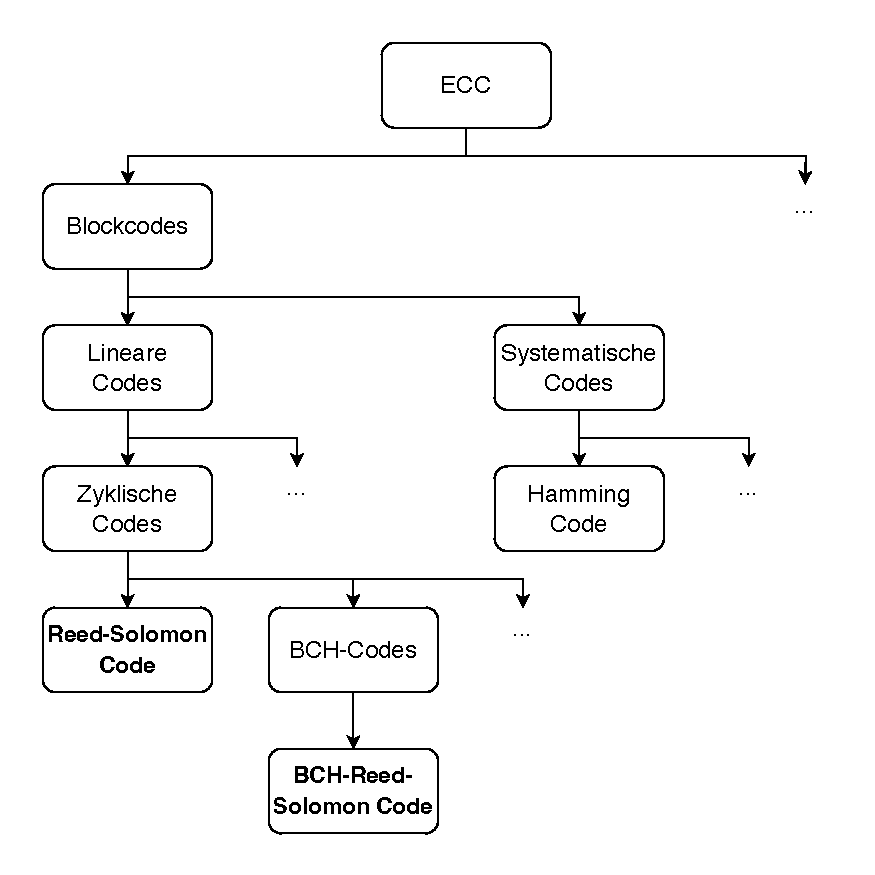
\includegraphics[width=0.8\textwidth]{figures/Codeklassen.drawio.pdf}
	\caption{Ausschnitt der Hierarchie von \acrshort{ecc}}
	\label{fig:eccHierarchy}
\end{figure}

Allerdings war fast 25 Jahre lang für das effektive Reed-Solomon-Verfahren kein effizienter Decodier\-algorithmus bekannt.
In der Zwischenzeit wurde aber weiter geforscht und -entwickelt.

1963 stellte J. J. Stone einen Reed-Solomon-Code vor, der auf dem Schema des \acrfull{bch}-Verfahrens von 1959 basiert \cite{petersonErrorcorrectingCodes1972}.
Trotz des Namens handelt es sich dabei aber um ein eigenständiges Verfahren, welches separat vom ursprünglichen Ansatz weiterentwickelt wurde (siehe Anhang \ref{app:bch-rs} auf Seite \pageref{app:bch-rs}).
Nachdem für die \acrshort{bch}-Codes 1969 ein effizienter Algorithmus, der so genannte Berlekamp-Massey-Algorithmus, gefunden wurde, war damit auch der Einsatz des auf dem \acrshort{bch}-Verfahren basierenden Reed-Solomon-Codes in der Praxis möglich \cite{berlekampNonbinaryBCHDecoding1968, masseyShiftregisterSynthesisBCH1969}.

Anwendung fand dieses Verfahrens zum ersten Mal im Jahr 1977 und zwar beim Voyager Programm der NASA \cite{wickerReedSolomonCodes1994}. 
Dadurch konnte eine robustere Kommunikation zwischen dem Raumfahrzeug und dem Raumfahrtkontrollzentrum bei einer großen Entfernung zur Erde gewährleistet werden \cite{ludwigVoyagerTelecommunications2002}.
Das erste kommerzielle, weit verbreitete und an den Endkunden gerichtete Produkt, in dem das Reed-Solomon-Verfahren eingesetzt wurde, war 1982 die \acrfull{cd} \cite{changReedSolomonProductCodeRSPC1998}.

Im Jahr 1986 ermöglichte der Berlekamp-Welch-Algorithmus die entscheidende Weiterentwicklung \cite{wendlingIntroductionReedSolomon2017}.
Entwickelt von Elwyn Berlekamp und Lloyd Welch verbesserte dieser Algorithmus die Effizienz des ursprünglichen Reed-Solomon-Schemas erheblich und förderte somit die Verbreitung der Reed-Solomon-Codes in verschiedenen Anwendungsbereichen. 
Eine detaillierte Beschreibung dieser findet sich in Kapitel \ref{ch:application} auf Seite \pageref{ch:application}.

Die kontinuierliche Weiterentwicklung und Anwendung der Reed-Solomon-Codes in verschiedenen Bereichen zeigt die Bedeutung und Vielseitigkeit dieses Fehlerkorrekturverfahrens. 
Um die Funktionsweise und die mathematischen Prinzipien dieses Codes in seiner Tiefe zu erfassen, ist es unabdingbar, sich mit den theoretischen Grundlagen auseinanderzusetzen. 
Im nächsten Kapitel werden daher die mathematischen Konzepte und Algorithmen erläutert, die dem Reed-Solomon-Code zugrunde liegen.